% Options for packages loaded elsewhere
\PassOptionsToPackage{unicode}{hyperref}
\PassOptionsToPackage{hyphens}{url}
%
\documentclass[
]{article}
\usepackage{amsmath,amssymb}
\usepackage{lmodern}
\usepackage{ifxetex,ifluatex}
\ifnum 0\ifxetex 1\fi\ifluatex 1\fi=0 % if pdftex
  \usepackage[T1]{fontenc}
  \usepackage[utf8]{inputenc}
  \usepackage{textcomp} % provide euro and other symbols
\else % if luatex or xetex
  \usepackage{unicode-math}
  \defaultfontfeatures{Scale=MatchLowercase}
  \defaultfontfeatures[\rmfamily]{Ligatures=TeX,Scale=1}
\fi
% Use upquote if available, for straight quotes in verbatim environments
\IfFileExists{upquote.sty}{\usepackage{upquote}}{}
\IfFileExists{microtype.sty}{% use microtype if available
  \usepackage[]{microtype}
  \UseMicrotypeSet[protrusion]{basicmath} % disable protrusion for tt fonts
}{}
\makeatletter
\@ifundefined{KOMAClassName}{% if non-KOMA class
  \IfFileExists{parskip.sty}{%
    \usepackage{parskip}
  }{% else
    \setlength{\parindent}{0pt}
    \setlength{\parskip}{6pt plus 2pt minus 1pt}}
}{% if KOMA class
  \KOMAoptions{parskip=half}}
\makeatother
\usepackage{xcolor}
\IfFileExists{xurl.sty}{\usepackage{xurl}}{} % add URL line breaks if available
\IfFileExists{bookmark.sty}{\usepackage{bookmark}}{\usepackage{hyperref}}
\hypersetup{
  hidelinks,
  pdfcreator={LaTeX via pandoc}}
\urlstyle{same} % disable monospaced font for URLs
\usepackage{longtable,booktabs,array}
\usepackage{calc} % for calculating minipage widths
% Correct order of tables after \paragraph or \subparagraph
\usepackage{etoolbox}
\makeatletter
\patchcmd\longtable{\par}{\if@noskipsec\mbox{}\fi\par}{}{}
\makeatother
% Allow footnotes in longtable head/foot
\IfFileExists{footnotehyper.sty}{\usepackage{footnotehyper}}{\usepackage{footnote}}
\makesavenoteenv{longtable}
\usepackage{graphicx}
\makeatletter
\def\maxwidth{\ifdim\Gin@nat@width>\linewidth\linewidth\else\Gin@nat@width\fi}
\def\maxheight{\ifdim\Gin@nat@height>\textheight\textheight\else\Gin@nat@height\fi}
\makeatother
% Scale images if necessary, so that they will not overflow the page
% margins by default, and it is still possible to overwrite the defaults
% using explicit options in \includegraphics[width, height, ...]{}
\setkeys{Gin}{width=\maxwidth,height=\maxheight,keepaspectratio}
% Set default figure placement to htbp
\makeatletter
\def\fps@figure{htbp}
\makeatother
\setlength{\emergencystretch}{3em} % prevent overfull lines
\providecommand{\tightlist}{%
  \setlength{\itemsep}{0pt}\setlength{\parskip}{0pt}}
\setcounter{secnumdepth}{-\maxdimen} % remove section numbering
\ifluatex
  \usepackage{selnolig}  % disable illegal ligatures
\fi

\author{}
\date{}

\begin{document}

\hypertarget{header-n0}{%
\section{CS305 Lab1 Report}\label{header-n0}}

11812418 樊青远

\hypertarget{header-n3}{%
\subsection{Q1}\label{header-n3}}

\begin{quote}
Use the ipconfig command to query the local ip, subnet mask, gateway,
MAC address, and screenshot instructions.
\end{quote}

\begin{verbatim}
>ifconfig
en0: flags=8863<UP,BROADCAST,SMART,RUNNING,SIMPLEX,MULTICAST> mtu 1500
	options=400<CHANNEL_IO>
	ether 38:f9:d3:75:70:88 
	inet6 fe80::472:9e7f:3642:1950%en0 prefixlen 64 secured scopeid 0xa 
	inet 10.17.120.246 netmask 0xffff8000 broadcast 10.17.127.255
	inet6 2001:da8:201d:1109::f762 prefixlen 128 dynamic 
	nd6 options=201<PERFORMNUD,DAD>
	media: autoselect
	status: active
\end{verbatim}

\begin{figure}
\centering
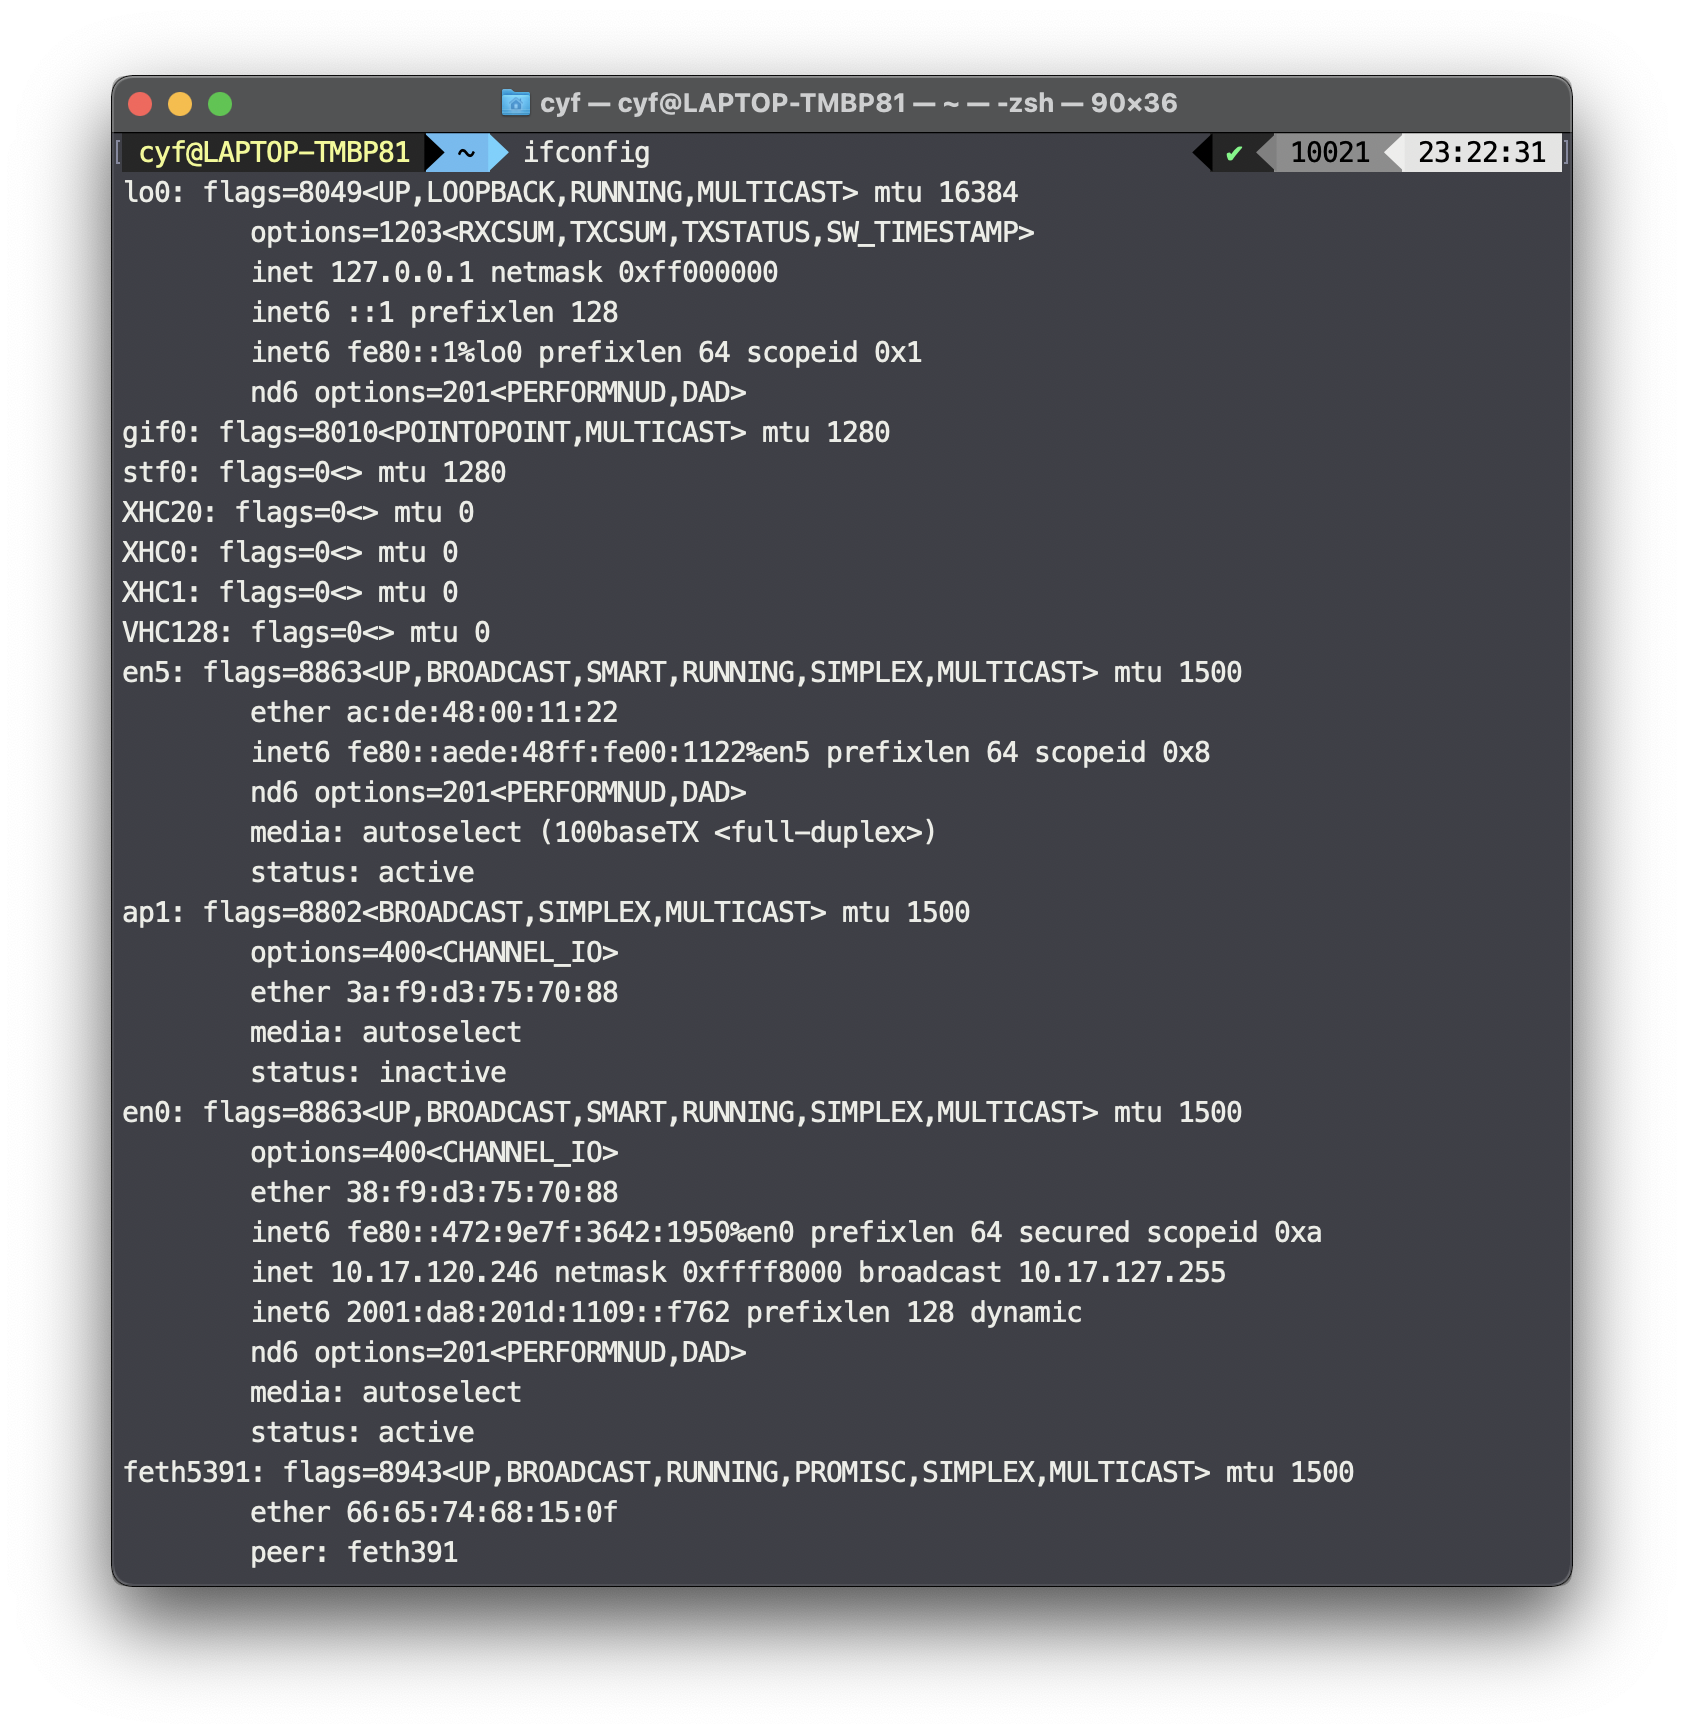
\includegraphics{/Users/cyf/OneDrive - 南方科技大学/UG/Course/T6/CS305B计算机网络B/lab/lab1/report/image-20210112233149752.png}
\caption{}
\end{figure}

\hypertarget{header-n8}{%
\subsubsection{Result}\label{header-n8}}

\begin{longtable}[]{@{}ll@{}}
\toprule
Parameters & Value \\ \addlinespace
\midrule
\endhead
Local IP & \texttt{10.17.120.246} \\ \addlinespace
Subnet mask & 0xffff8000 (\texttt{255.255.128.0}) \\ \addlinespace
Gateway & \texttt{10.17.127.255} \\ \addlinespace
MAC address & \texttt{38:f9:d3:75:70:88} \\ \addlinespace
\bottomrule
\end{longtable}

\hypertarget{header-n26}{%
\subsection{Q2}\label{header-n26}}

\begin{quote}
Ping www.baidu.com and ping www.sustc.edu.cn, the screenshot gives a
brief description of the echo message (whether the destination host is
reachable, the communication duration, the TTL value)
\end{quote}

\hypertarget{header-n29}{%
\subsubsection{ping www.baidu.com}\label{header-n29}}

\begin{verbatim}
>ping www.baidu.com
PING www.a.shifen.com (14.215.177.38): 56 data bytes
64 bytes from 14.215.177.38: icmp_seq=0 ttl=54 time=7.229 ms
64 bytes from 14.215.177.38: icmp_seq=1 ttl=54 time=20.660 ms
64 bytes from 14.215.177.38: icmp_seq=2 ttl=54 time=9.278 ms
64 bytes from 14.215.177.38: icmp_seq=3 ttl=54 time=25.890 ms
^C
--- www.a.shifen.com ping statistics ---
4 packets transmitted, 4 packets received, 0.0% packet loss
round-trip min/avg/max/stddev = 7.229/15.764/25.890/7.769 ms
\end{verbatim}

\hypertarget{header-n31}{%
\paragraph{Screenshot}\label{header-n31}}

\begin{figure}
\centering
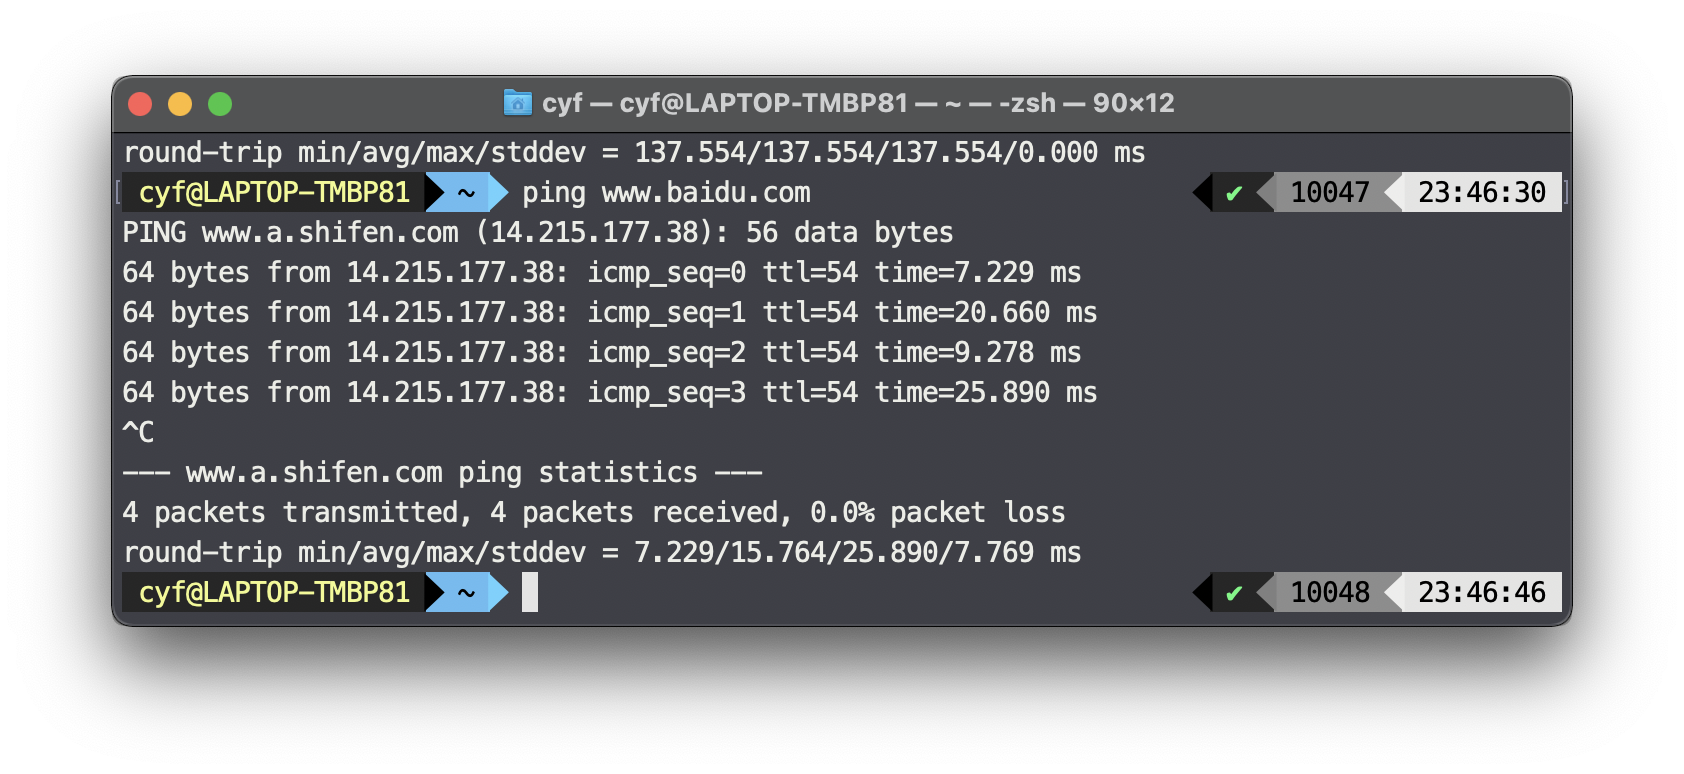
\includegraphics{/Users/cyf/OneDrive - 南方科技大学/UG/Course/T6/CS305B计算机网络B/lab/lab1/report/image-20210112234651895.png}
\caption{}
\end{figure}

\hypertarget{header-n33}{%
\subsubsection{ping www.sustc.edu.cn}\label{header-n33}}

\begin{verbatim}
>ping www.sustc.edu.cn
PING www.sustc.edu.cn (172.18.8.244): 56 data bytes
64 bytes from 172.18.8.244: icmp_seq=0 ttl=62 time=2.850 ms
64 bytes from 172.18.8.244: icmp_seq=1 ttl=62 time=21.632 ms
64 bytes from 172.18.8.244: icmp_seq=2 ttl=62 time=21.563 ms
64 bytes from 172.18.8.244: icmp_seq=3 ttl=62 time=10.690 ms
^C
--- www.sustc.edu.cn ping statistics ---
4 packets transmitted, 4 packets received, 0.0% packet loss
round-trip min/avg/max/stddev = 2.850/14.184/21.632/7.915 ms
\end{verbatim}

\hypertarget{header-n35}{%
\paragraph{Screenshot}\label{header-n35}}

\begin{figure}
\centering
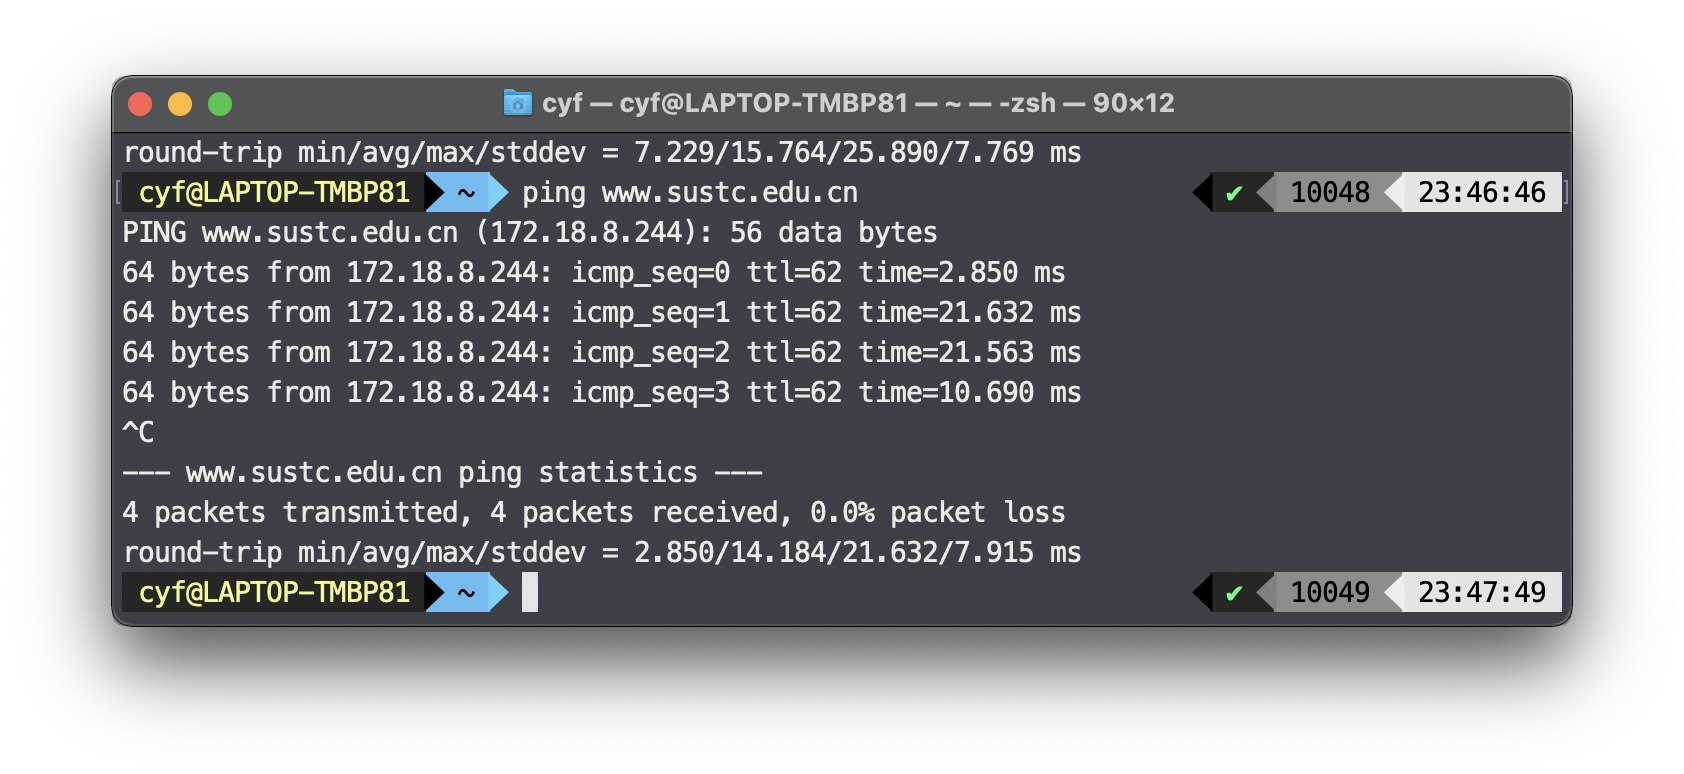
\includegraphics{/Users/cyf/OneDrive - 南方科技大学/UG/Course/T6/CS305B计算机网络B/lab/lab1/report/image-20210112234755159.png}
\caption{}
\end{figure}

\hypertarget{header-n37}{%
\subsection{Q3}\label{header-n37}}

\begin{quote}
Use the netstat command to check the traffic statistics on the local
Ethernet card and take a screenshot
\end{quote}

\begin{figure}
\centering
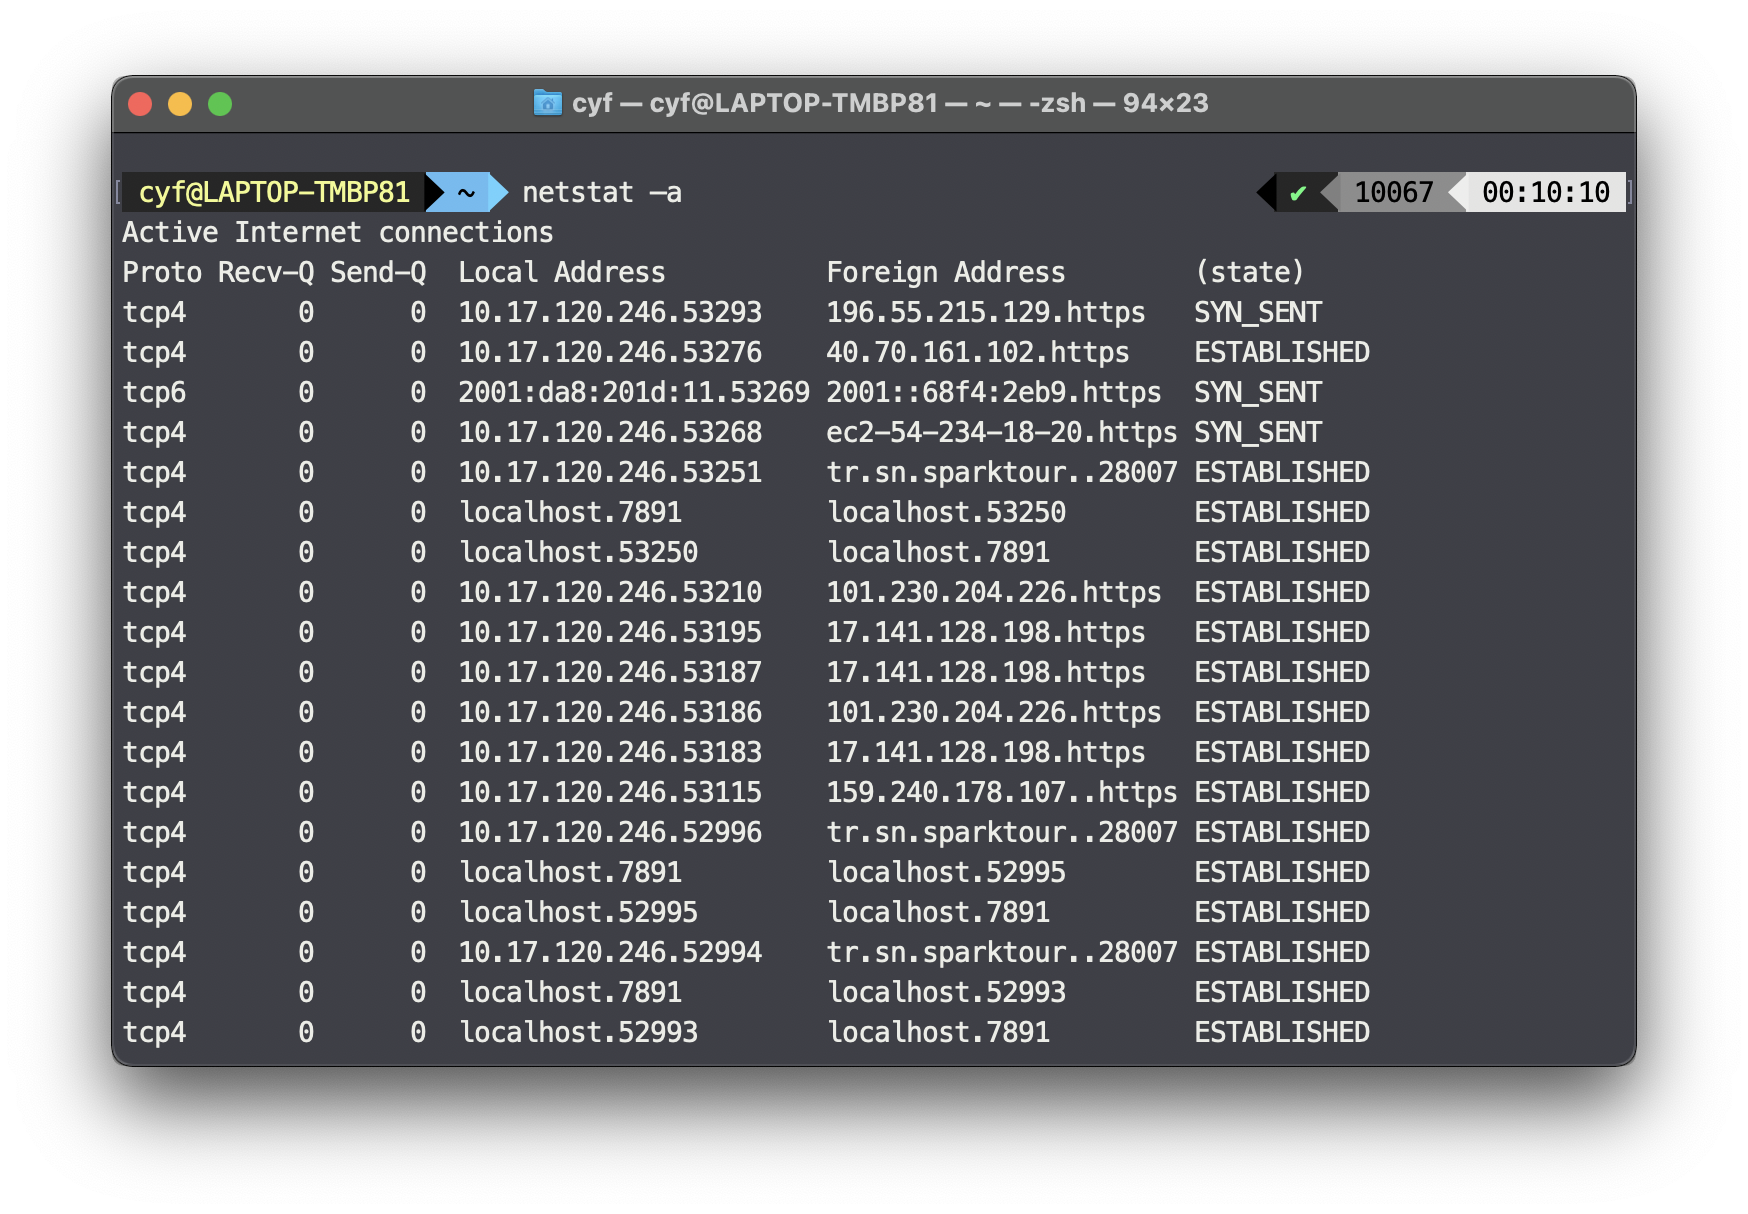
\includegraphics{/Users/cyf/OneDrive - 南方科技大学/UG/Course/T6/CS305B计算机网络B/lab/lab1/report/image-20210113001153688.png}
\caption{}
\end{figure}

\hypertarget{header-n41}{%
\subsection{Q4}\label{header-n41}}

\begin{quote}
Use the tracert command to access www.baidu.com and take a screenshot
analysis to mark the total number of hops from the host to the
destination host, whether there is any icmp packet loss, and the ip
address of the server where www.baidu.com is located.
\end{quote}

\begin{figure}
\centering
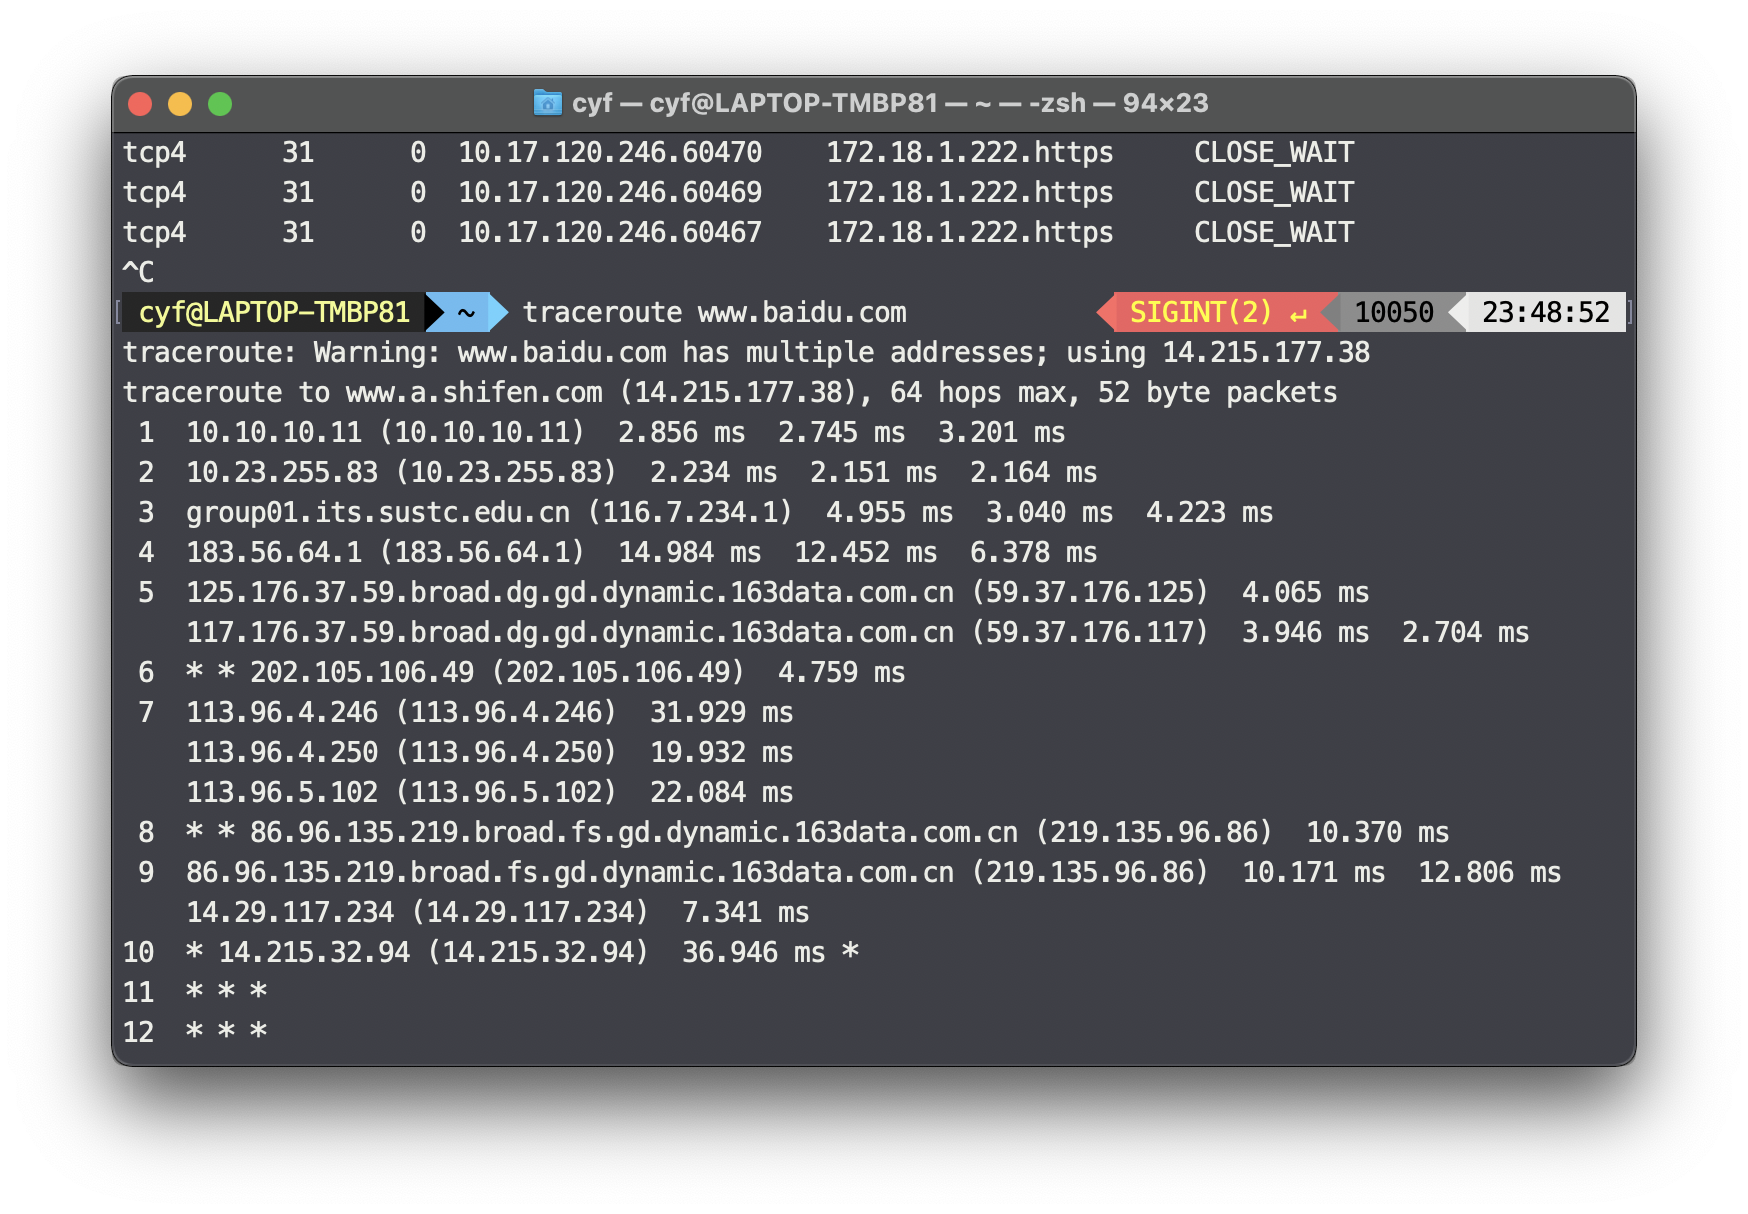
\includegraphics{/Users/cyf/OneDrive - 南方科技大学/UG/Course/T6/CS305B计算机网络B/lab/lab1/report/image-20210113000705782.png}
\caption{}
\end{figure}

\hypertarget{header-n45}{%
\subsection{Q5}\label{header-n45}}

\begin{quote}
In this lab class, list the commands that requires addition parameters
to run. Use these commands and parameters (each command chooses 2 or 3
of them to experiment), take a screensho
\end{quote}

\hypertarget{header-n48}{%
\subsubsection{ping}\label{header-n48}}

\begin{verbatim}
usage: ping [-AaDdfnoQqRrv] [-c count] [-G sweepmaxsize]
            [-g sweepminsize] [-h sweepincrsize] [-i wait]
            [-l preload] [-M mask | time] [-m ttl] [-p pattern]
            [-S src_addr] [-s packetsize] [-t timeout][-W waittime]
            [-z tos] host
       ping [-AaDdfLnoQqRrv] [-c count] [-I iface] [-i wait]
            [-l preload] [-M mask | time] [-m ttl] [-p pattern] [-S src_addr]
            [-s packetsize] [-T ttl] [-t timeout] [-W waittime]
            [-z tos] mcast-group
Apple specific options (to be specified before mcast-group or host like all options)
            -b boundif           # bind the socket to the interface
            -k traffic_class     # set traffic class socket option
            -K net_service_type  # set traffic class socket options
            -apple-connect       # call connect(2) in the socket
            -apple-time          # display current time
\end{verbatim}

\texttt{ping\ -c} means the count the \texttt{ping} command runs. e.g.
\texttt{ping\ -c\ 10\ 1.2.4.8}

\begin{figure}
\centering
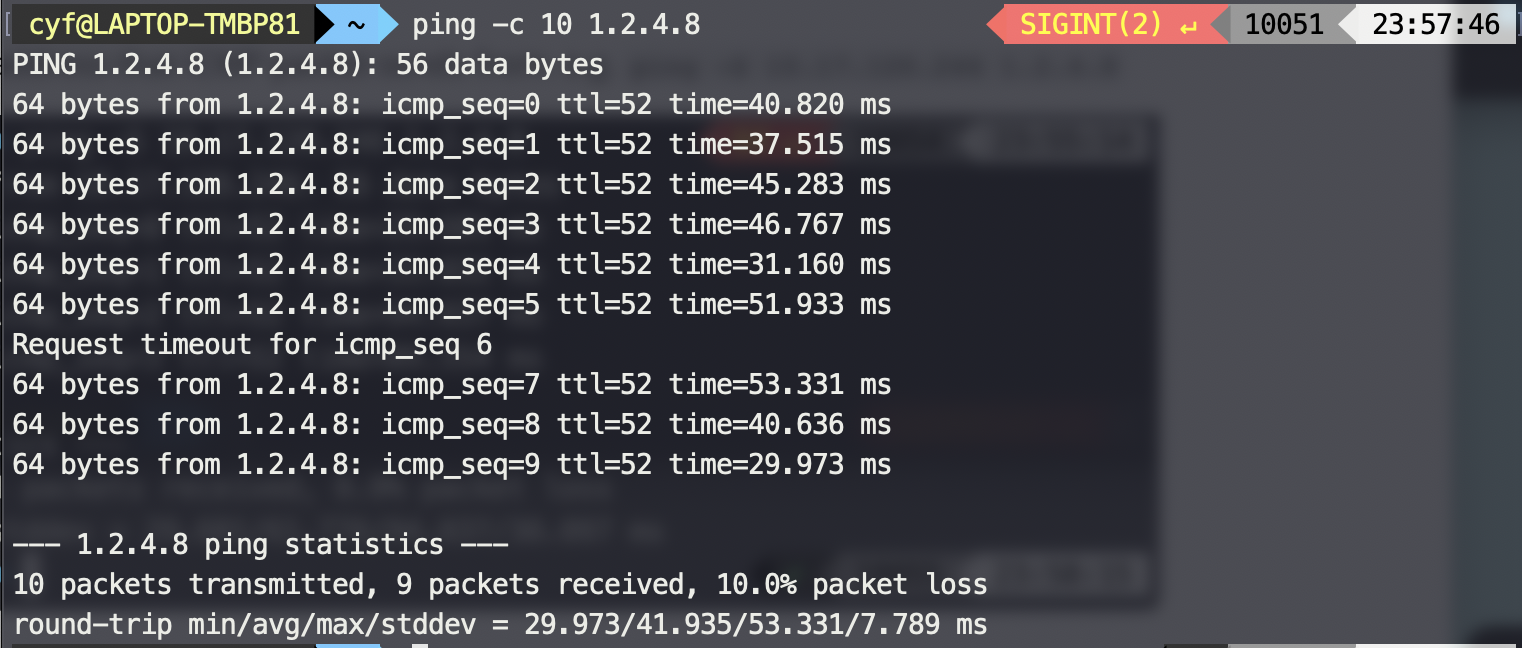
\includegraphics{/Users/cyf/OneDrive - 南方科技大学/UG/Course/T6/CS305B计算机网络B/lab/lab1/report/image-20210112235920182.png}
\caption{}
\end{figure}

\texttt{ping\ -S} means specific the address that ICMP packet sends
from. e.g. \texttt{ping\ -S\ 10.17.120.246\ 1.2.4.8}

\begin{figure}
\centering
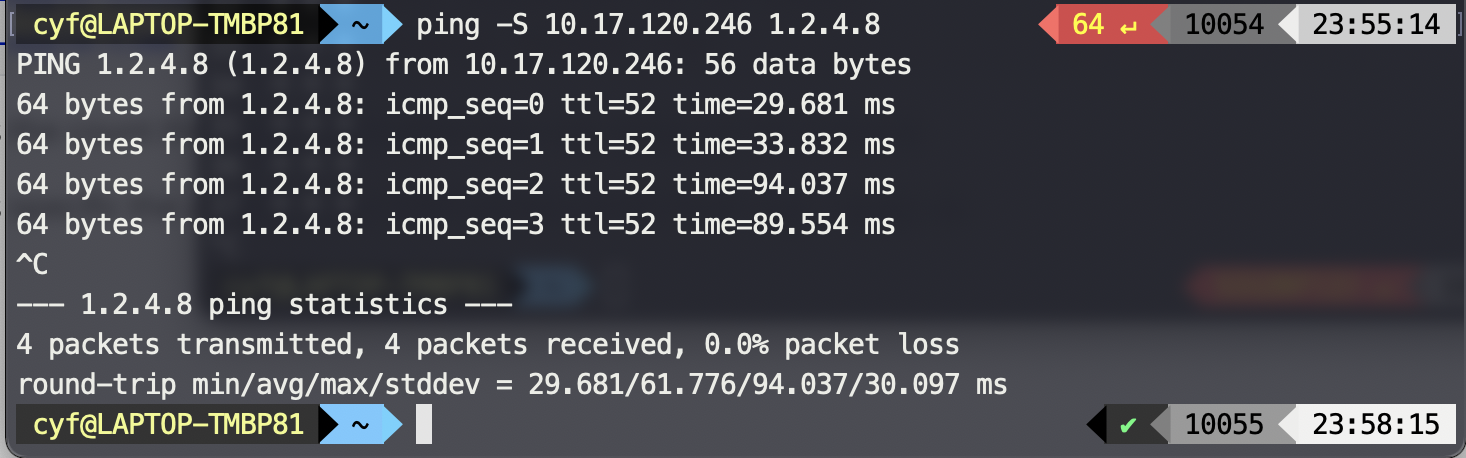
\includegraphics{/Users/cyf/OneDrive - 南方科技大学/UG/Course/T6/CS305B计算机网络B/lab/lab1/report/image-20210112235828415.png}
\caption{}
\end{figure}

\hypertarget{header-n54}{%
\subsubsection{Traceroute}\label{header-n54}}

\begin{verbatim}
Version 1.4a12+Darwin
Usage: traceroute [-adDeFInrSvx] [-A as_server] [-f first_ttl] [-g gateway] [-i iface]
	[-M first_ttl] [-m max_ttl] [-p port] [-P proto] [-q nqueries] [-s src_addr]
	[-t tos] [-w waittime] [-z pausemsecs] host [packetlen]
\end{verbatim}

\texttt{traceroute\ -i} means traceroute using the specific interface.
e.g. \texttt{traceroute\ -i\ en0\ 1.0.0.1}

\begin{figure}
\centering
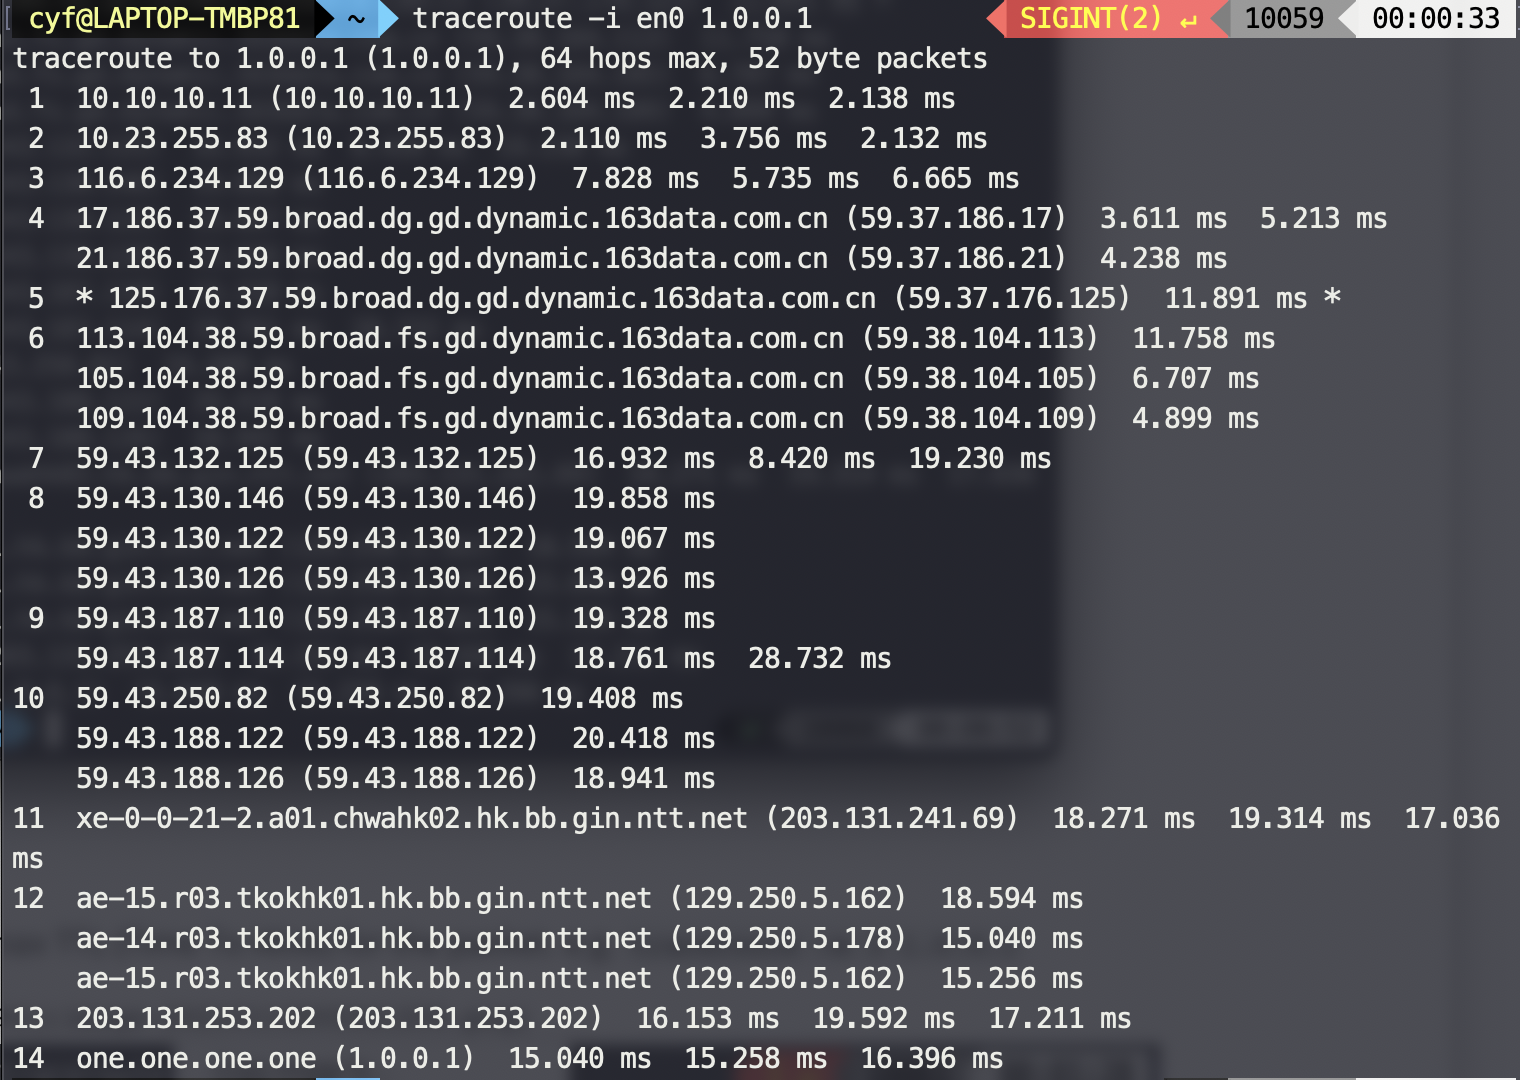
\includegraphics{/Users/cyf/OneDrive - 南方科技大学/UG/Course/T6/CS305B计算机网络B/lab/lab1/report/image-20210113000352011.png}
\caption{}
\end{figure}

\texttt{traceroute\ -m} specific the max TTL (Time To Live) for the
packet. e.g. \texttt{traceroute\ -m\ 3\ 1.0.0.1}

\begin{figure}
\centering
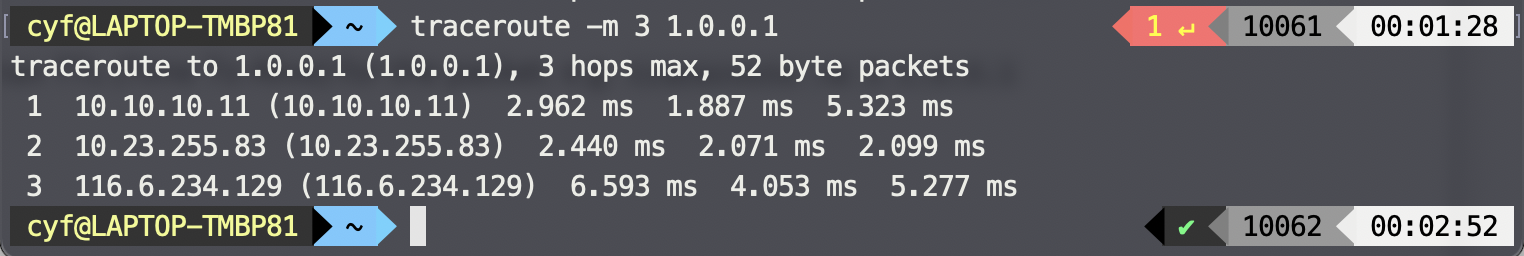
\includegraphics{/Users/cyf/OneDrive - 南方科技大学/UG/Course/T6/CS305B计算机网络B/lab/lab1/report/image-20210113000341294.png}
\caption{}
\end{figure}

\hypertarget{header-n60}{%
\subsubsection{Nslookup}\label{header-n60}}

\texttt{nslookup\ -query=AAAA\ www.cloudflare.com\ 172.18.1.92} means
query the \texttt{AAAA} record of \texttt{www.cloudflare.com} from DNS
server \texttt{172.18.1.92}.

\begin{figure}
\centering
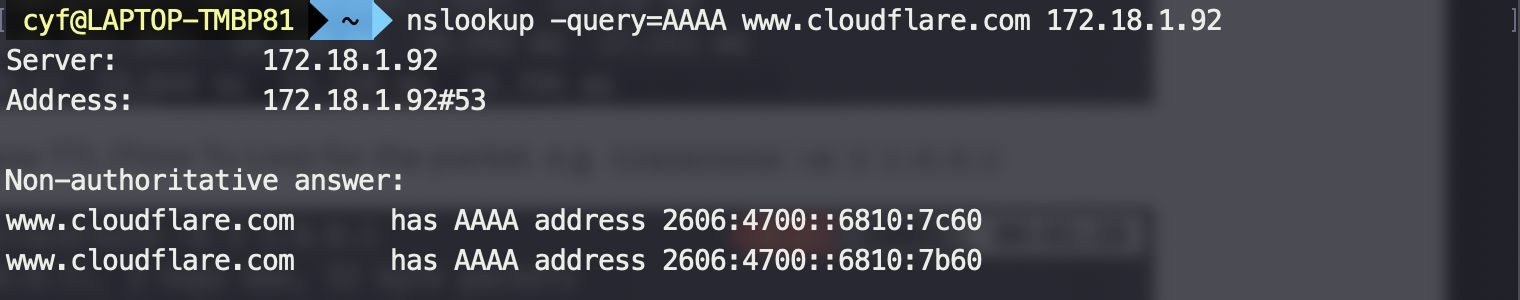
\includegraphics{/Users/cyf/OneDrive - 南方科技大学/UG/Course/T6/CS305B计算机网络B/lab/lab1/report/image-20210113000814949.png}
\caption{}
\end{figure}

\texttt{nslookup\ -query=TXT\ xn-\/-g28h.hack.ustclug.org\ 172.18.1.92}
means query the \texttt{AAAA} record of
\texttt{xn-\/-g28h.hack.ustclug.org} from DNS server
\texttt{172.18.1.92}.

\begin{figure}
\centering
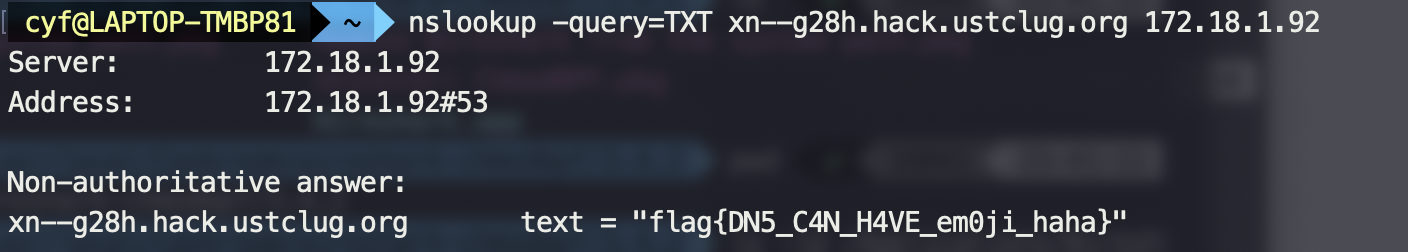
\includegraphics{/Users/cyf/OneDrive - 南方科技大学/UG/Course/T6/CS305B计算机网络B/lab/lab1/report/image-20210113001019382.png}
\caption{}
\end{figure}

\end{document}
